\documentclass{ExcelAtFIT}
%\documentclass[czech]{ExcelAtFIT} % when writing in CZECH
%\documentclass[slovak]{ExcelAtFIT} % when writing in SLOVAK


%--------------------------------------------------------
%--------------------------------------------------------
%	REVIEW vs. FINAL VERSION
%--------------------------------------------------------

%   LEAVE this line commented out for the REVIEW VERSIONS
%   UNCOMMENT this line to get the FINAL VERSION
\ExcelFinalCopy


%--------------------------------------------------------
%--------------------------------------------------------
%	PDF CUSTOMIZATION
%--------------------------------------------------------

\hypersetup{
	pdftitle={Real Time Data Processing with Strimzi Project},
	pdfauthor={Maroš Orsák},
	pdfkeywords={Clustering, Real time data processing, Strimzi, Apache Kafka, Quarkus, super-sonic \& sub-atomic java, Kubernetes}
}

\lstset{ 
	backgroundcolor=\color{white},   % choose the background color; you must add \usepackage{color} or \usepackage{xcolor}; should come as last argument
	basicstyle=\footnotesize\tt,        % the size of the fonts that are used for the code
}

%--------------------------------------------------------
%--------------------------------------------------------
%	ARTICLE INFORMATION
%--------------------------------------------------------

\ExcelYear{2020}

\PaperTitle{Real Time Data Processing with Strimzi Project}

\Authors{Maroš Orsák*}
\affiliation{*%
  \href{mailto:xokrsa02@fit.vutbr.cz}{xorsak02@fit.vutbr.cz},
  \textit{Faculty of Information Technology, Brno University of Technology}}
%%%%--------------------------------------------------------
%%%% in case there are multiple authors, use the following fragment instead
%%%%--------------------------------------------------------
%\Authors{Jindřich Novák*, Janča Dvořáková**}
%\affiliation{*%
%  \href{mailto:xnovak00@stud.fit.vutbr.cz}{xnovak00@stud.fit.vutbr.cz},
%  \textit{Faculty of Information Technology, Brno University of Technology}}
%\affiliation{**%
%  \href{mailto:xdvora00@stud.fit.vutbr.cz}{xdvora00@stud.fit.vutbr.cz},
%  \textit{Faculty of Information Technology, Brno University of Technology}}

\Keywords{Clustering, Real time data processing, Strimzi, Apache Kafka, Quarkus, super-sonic \& sub-atomic java, Kubernetes}

\Supplementary{ --- \href{https://github.com/see-quick/bachelor-thesis}{Downloadable Code}}


%--------------------------------------------------------
%--------------------------------------------------------
%	ABSTRACT and TEASER
%--------------------------------------------------------

\Abstract{
Container technologies become broadly used in modern times. In prevailing, applications made on the micro-service architecture are rising. This paper analyzes the design of an app that will process data in real-time. Further, the application will be built using state-of-the-art technologies used by world companies like Netflix, Uber. They are using the systems for real-time data processing such as Apache Kafka, and in recent times they raised it on a higher level by encapsulating this system in the container environment, which guaranteeing effortless scalability. Additionally, using the latest native Kubernetes technologies for processing dozens of data with Quarkus and Strimzi. The problem, which arises, is that these types of real-time data processing systems encapsulated in the containers are especially challenging to test. This paper will also show the designed long term test of the application and Strimzi system, also known as Marathon, which is the ideal demonstration of user conditions.}

%--------------------------------------------------------
%--------------------------------------------------------
%--------------------------------------------------------
%--------------------------------------------------------
\begin{document}

\startdocument


%--------------------------------------------------------
%--------------------------------------------------------
%	ARTICLE CONTENTS
%--------------------------------------------------------

%--------------------------------------------------------
%--------------------------------------------------------
%--------------------------------------------------------
%--------------------------------------------------------
\section{Introduction}

Clustering has become a commonly used word. The era of containers proliferates by creating container orchestral. Data is all around us without noticing them, but how are we able to test such an application based on these technologies? How are we able to simulate user load environment in these kinds of systems? We will find the answer in the following subsections.

Strimzi supplies an idea of how to run Apache Kafka cluster inside the Kubernetes cluster in multiple ways. First of all, there is no simple way to simulate existing traffic with the Strimzi project. Apache Kafka is a distributed messaging system used for building real-time processing data. Kubernetes is a container orchestral, which makes work with virtual units handy and so easy to manage instead of having only container engines. The designed system will be used as a component for testing the Strimzi application, in real scenarios with an enormous load of data. Moreover, tested in a long term environment to guarantee that Strimzi is a stable system.

On this type of problem currently, we have three types of explications. All of them have some advantages and disadvantages. Firstly, we can take a look at this problem that we do not need to create our external system and use some that are already created. Tremendously, we have saved much time, but what are we missing in this? At first glance, this option can look magnificent, but what if we decide to extend our testing scenarios, but with this unknown black box code, we will be unable to do it. This factor must take place into consideration. The second alternative is to adapt to some available system and fork it and then extend it. Also, we can save some time on that instead of creating it from scratch.
Nevertheless, it can sometimes be excruciating to look at some unknown code, which is not written by your hands and can hide many severe errors, which is not visibly in the first place. Ultimately, you clever one know that if we create our system, we spare much time fixing some other bugs, plus we can extend it very smoothly. In other words, creating our testing application, which will represent user conditions in a big load, will be the best choice we can ever do.

As described in the previous paragraph, our solution is to create our external system to test Strimzi entirely and be able to modifiable in a short period. We will use state-of-art technologies for micro-service architecture, which is Quarkus and React \cite{React}. Quarkus will have the responsibility to generate load and fill this data to the Strimzi. Moreover, in the second phase, it will retrieve this data from aggregate. After the aggregation phase is over, Quarkus will expose these sets of data to the React. React is just extension, to be visible for a tester that data are changing. The main priority has Quarkus with sending and aggregating data from Strimzi. 

The case study, which we picked, is air pollution. Initially, that was picked because we had real data providing by IoT sensors in Newcastle, but we found out that if we want to create some load, this data has to synthesize with some generator. In the following figure \ref{fig:strimziWithExternalSystem}, we can see the abstract view of communication between the external system and Strimzi, which are encapsulated inside the Kubernetes cluster.

\begin{figure}[h!]
	\centering
	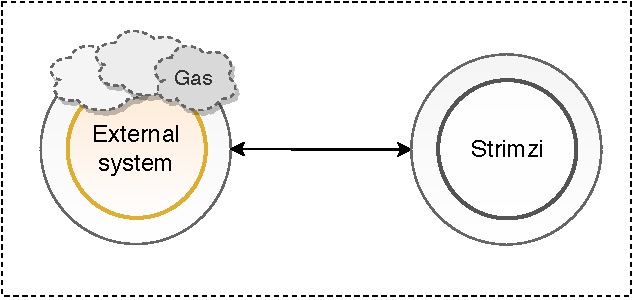
\includegraphics[width=1\linewidth]{images/01-introduction/TitleForArticleWithColor.pdf}
	\caption{Strimzi with the external system, encapsulated in the Kubernetes cluster}
	\label{fig:strimziWithExternalSystem}
\end{figure}


%--------------------------------------------------------
%--------------------------------------------------------
%--------------------------------------------------------
%--------------------------------------------------------
\section{Strimzi}
\label{sec:HowToUse}

The first thing if we want to understand what Strimzi is, we must first get in touch with Apache Kafka and Kubernetes. Nowadays, applications are based on a cloud environment or we want to be as we called a cloud-native and Kafka is not an exception. We might ask what Kafka and how to make it cloud-native ? Some of you could think what can be created using Kubernetes and Apache Kafka technologies? The answer to these questions is a system called Strimzi\footnote{Set of operators for deploying Kafka into Kubernetes cluster - \url{https://strimzi.io/}}.

\subsection{Kubernetes}

The idea of the containers was published far in the past. The primary purpose of this technology is to be platform-independent and scalable. Moreover, it is an abstraction of the application layer. It does not create a virtual machine but uses the kernel of the physical computer and creates virtualization for the application and library needed. We have also known as lightweight compared to virtual machines. These days is that alternative suitable for agile development.

The underlying architecture of Kubernetes \cite{Kubernetes} is based on master and slave. The Master's node responsibility is to ensure that every slave node has access to a kube-apiserver, which is making all REST API delegating all calls to the kubelet. On the other hand, we have slave nodes where we have our running applications inside pods and controlling by some Kubernetes controllers such as \emph{Deployment}, \emph{ReplicaSet}, or \emph{Statefulset}.  

Furthermore, the following terminology is also needed to understand Kubernetes in the simplest possible way:
\begin{itemize}
 \item \textbf{kube-apiserver} \---\ validates and configures data for the API objects such as pods, services, replication controllers, and more. REST operations do everything.
   \item \textbf{pod} \---\  is the smallest unit that can contain application in its container, which can be deployed inside the Kubernetes cluster. Inside the pod, we can find one or more containers where they share storage, network, and a specification for how to run the containers. It is considered as a leading resource of the Kubernetes REST API. As an example of the pod, we can image Kafka running inside pod's container, which can serve as default Kafka actions like store messages in topics.
  \item \textbf{deployment} \---\   act as managers, which taking care of identical pods, and for this reason, they are known as controllers. Without having deployments, it would be tough to manage many pods. As an example, we can imagine the following scenario: 
  The application will be released, so with that, we assume that the new image will be available. Only one responsibility would change the image name inside the deployment file and confirm that with \emph{kubectl apply -f deployment-definition.yaml}. It will trigger the rolling update, and your application will be upgraded from one version to another without the user having any clue that something behind the scene is changing. Of course, the precondition is that you have at least two replicas of your application running.
 \item \textbf{service} \---\  are considered as a object, which represents communication between nodes, for instance, between two pods. Kubernetes has a type of Cluster IP, which means that communication can be established only inside of the Kubernetes cluster. The way how you will be able to expose your application outside of the cluster will be to use the following type of service, which Kubernetes offers, for instance, Nodeport, Load-balancer, or with Ingress.
 \item \textbf{custom resources} \---\  is the extension of the Kubernetes API. Simply imaginable as many defined objects that will serve to our created application using CRUD rules. The definition of these objects is in stateless YAML files. For instance, we can define our custom resources, which we called CRDs; in other words, \emph{Custom resource definitions}. As an administrator of the cluster, you can apply these files to have it in your Kubernetes cluster.
\end{itemize}

What is worth mentioning is that every single Kubernetes object is defined with a stateless YAML file. For instance, this is my definition of the deployment load-generator component \href{https://github.com/see-quick/bachelor-thesis/blob/master/install/01-quarkus-load-generator-deployment.yaml}{deployment example}. Following figure \ref{fig:strizmi:kubernetesDeploy} illustrating steps what is needed to deploy some application to the Kubernetes environment. Besides ignoring, we have already set up cluster and download CLI, and we need to create a stateless file. This file applies via command, and afterward, Kubernetes will take care of creating a deployment, which will trigger the creation of pod.

\begin{figure}[h!]
	\centering
	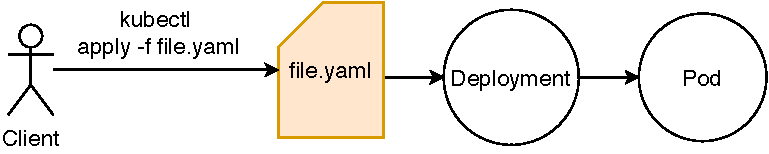
\includegraphics[width=1\linewidth]{images/02-strimzi/applyCommandBigh.pdf}
	\caption{Common objects with Kubernetes client}
	\label{fig:strizmi:kubernetesDeploy}
\end{figure}

\subsection{Apache Kafka} 

Apache Kafka\cite{Kafka} is a distributed streaming platform that offers many features like high performance, distribution, commit log service, and more. It publishes and subscribes to record streams that are similar to a message queue or enterprise messaging system. Moreover, store record streams in a robust, fault-tolerant way. What is more, Kafka\cite{KafkaBook} creates real-time data flows that reliably capture data between systems or applications and lastly, used for real-time streaming applications that transform or respond to data streams. Additionally, widely used by many big companies like LinkedIn, Spotify, Uber, and more.

Assume example, where we have five source systems and five target systems. Each source system needs something from the target system, so in that case, we have twenty-five links, which is not effective. You may have noticed that this is a quadratic complexity. That's why Kafka was born by developers from LinkedIn. If we illustrate the same example with ten systems and Kafka will serve as Middleware. In that case, each source system will be bind to the Kafka broker and all data will be delivered to target systems with only one link. The following figure \ref{fig:externalSystem:kafkaReduceDependency} illustrating described idea.

\begin{figure*}[h!t]
	\centering
	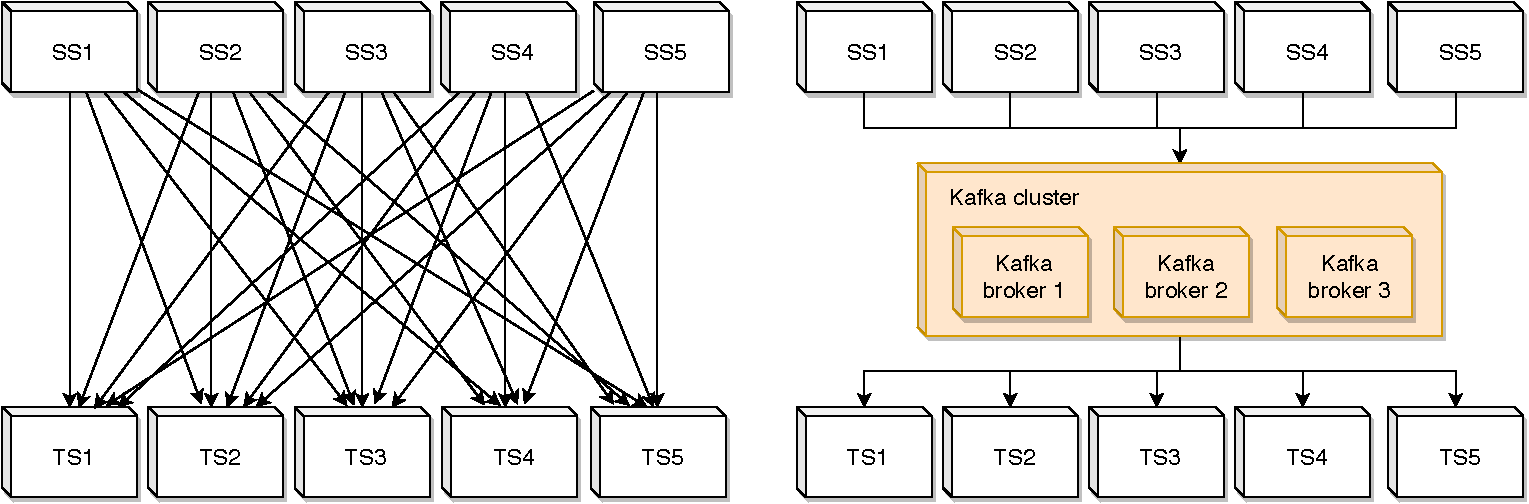
\includegraphics[width=0.9\linewidth]{images/02-strimzi/KafkaReduceDependencyBig.pdf}
	\caption{Kafka reduces dependency between source and target systems}
	\label{fig:externalSystem:kafkaReduceDependency}
\end{figure*}

Same as we applied for the Kubernetes we need to describe some core concepts of Kafka and they are as follows:
\begin{itemize}
    \item \textbf{kafka broker} \---\ Kafka server, Kafka node, or Kafka broker. Not one person would have been confused by these names. All of these names refer to the same concept. Kafka broker is a server application, which taking care of all the data, that was published into the Kafka cluster. By contrast, consumers can fetch data from a specific topic. Kafka broker can be scaled to more that one unit, and it is encapsulated in how we called the Kafka cluster. More about it in the following subsection.
	\item \textbf{producer} \---\ we understand producer as application, which publishes messages into Kafka broker. Moreover, his responsibilities are to make sure that he binds to the correct topic on a specific partition. Known, techniques are round-robin, where the producer will publish messages to that partition, which is not so active or do it by some self partition method based on the hash table algorithm.
	\item \textbf{consumer} \---\ we understand consumer who subscribes to Kafka broker with a specific topic and receives all the data from it. The method that consumers using is called polling6. For the most situation data is read for each partition. We will discuss the topic and partitions in follow up sub-sections.
 	\item \textbf{topic} \---\ The best description of the topic is by giving an example. I ensure that we know what a database table is so the equivalence in Kafka is Topic as an illustration in figure 2.8. We can not change or update the data if it has already been published. The topic consists of partitions. Messages are being stored on a specific topic.
\end{itemize}

These four topics we can illustrate in the figure \ref{fig:strizmi:consumerProducerTopicKafka} describing the simple scenario. 

\begin{figure}[h!]
	\centering
	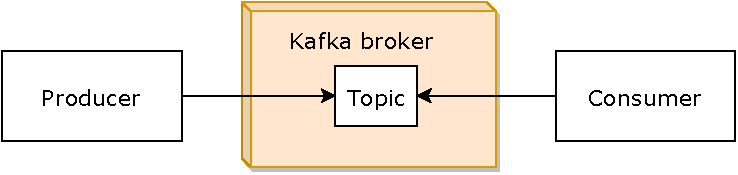
\includegraphics[width=1\linewidth]{images/02-strimzi/KafkaConsumerProducerBig.pdf}
	\caption{Kafka broker with consumer and producer}
	\label{fig:strizmi:consumerProducerTopicKafka}
\end{figure}

All of the learned concepts in the previous subsections 2.1 and 2.2 were necessarily known for a simple reason. If you imagine the power of Kafka within a bare-metal server and add the attributes of the Kubernetes container orchestral, this can give you the ability to build an application. The system called Strimzi. The whole concept is designed by Operators. Every operator has his custom resources definitions with which he handles objects created by custom resources. His primary responsibility is to take care of the application. Entity Operator just encapsulates two essential operators, which manage topics and users inside the Kubernetes. On the following \ref{fig:strizmi:architecture} example, you can see previously described behavior

\begin{figure}[h!]
	\centering
	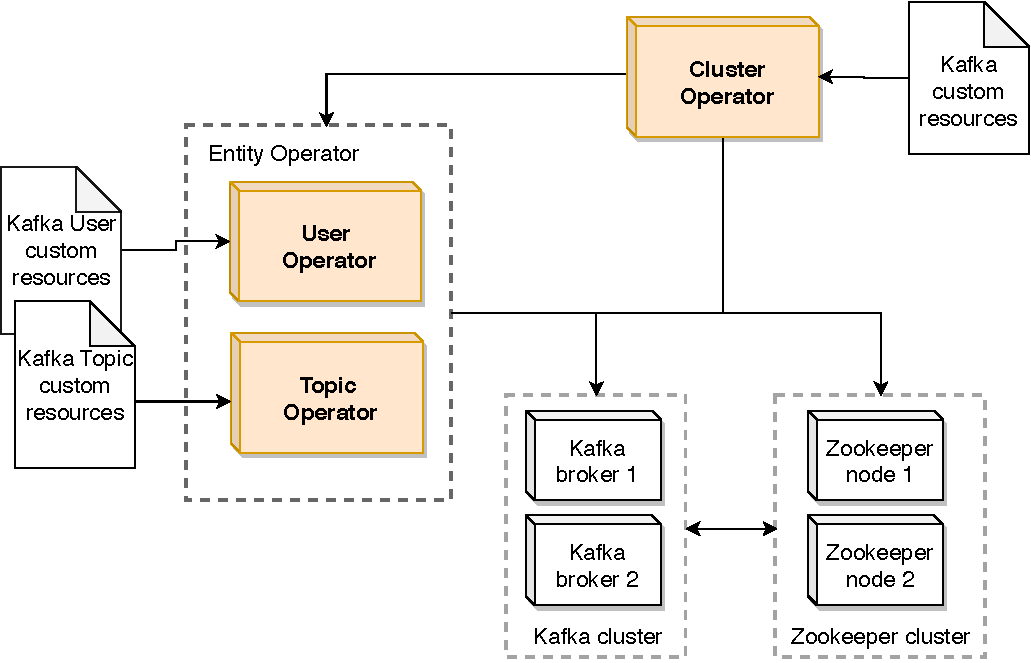
\includegraphics[width=1\linewidth]{images/02-strimzi/StrimziArchitectureBig.pdf}
	\caption{Strimzi architecture}
	\label{fig:strizmi:architecture}
\end{figure}

The second thing we need to understand if we want to create our application, which will process dozens of records in a short period, is to have some in-memory storage. This storage must satisfy the following requirements. \begin{itemize} 
  \item \textbf{fault-tolerance} \---\ we do not want that some data will be lost in critical systems, even if we are talking about some messaging-based platforms, which are not so critical on human life but if we send some message we want that message to be delivered to the receiver.
  \item \textbf{velocity} \---\ we live at a time when we all need things fast and right, Strimzi is built on top the Kafka, which can process millions of records and immediately respond.
  \item \textbf{scalability} \---\ specifically horizontal scalability using to distribute load between replicated applications
\end{itemize}

%--------------------------------------------------------
%--------------------------------------------------------
%--------------------------------------------------------
%--------------------------------------------------------


\section{External system with Strimzi}
\label{sec:externalSystem}

The whole concept of this application is to have separated logical units, which will communicate over services, also known as microservice architecture. Firstly it is Quarkus \cite{Quarkus}. It was created because with the big bang of cloud-native applications and microservices architecture, where start up time of the application, memory, and CPU consumption matters. All these aspects are essential, and that is why this technology was made to replace old Java. Framework with name Quarkus. In case of interest, you can find more about Quarkus \href{https://quarkus.io/}{here}. Secondly, we used for the frontend of the application React.  Created by the Facebook community and mainly by software engineer Jordan Walke written in Javascript language. Sometimes by non-specialists described as a framework. Javascript library, superset for the Javascript. It is widely used for developing SPA\footnote{single page applications}. This all can be referred to as React.

\begin{figure}[h!]
	\centering
	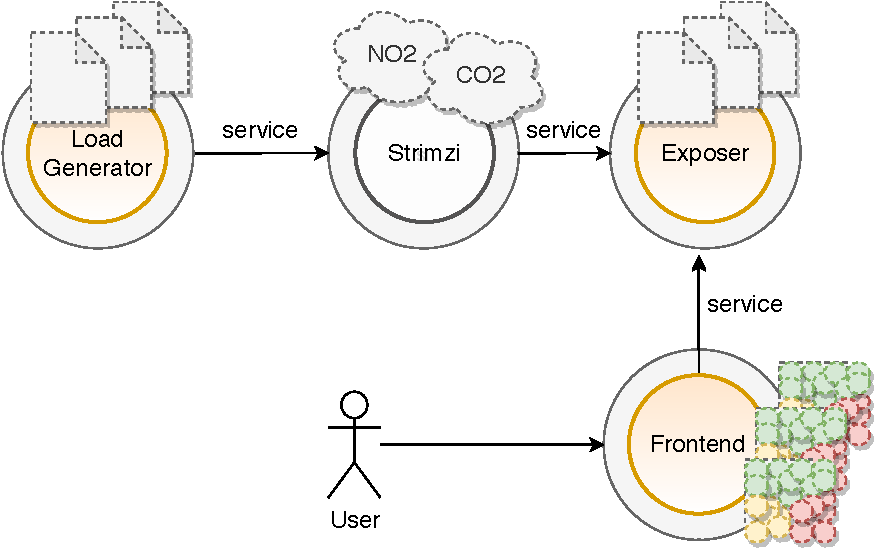
\includegraphics[width=1\linewidth]{images/03-externalSystem/ApplicationWithStrimziOrange.pdf}
	\caption{Design of external system with Strimzi}
	\label{fig:externalSystem:design}
\end{figure}

We can divide this application to 4 components as you can see in the figure \ref{fig:externalSystem:design}:
\begin{itemize}
	\item \textbf{load generator} \---\ quarkus application for generating load to the Strimzi.
	\item \textbf{strimzi} \---\ strimzi system, which represents encapsulated kafka, which processing data generated by load generator and ensuring fault-tolerance.
	\item \textbf{exposer} \---\ quarkus application responsible for the aggregation of data and exposing them to REST API endpoint to be accessible from React.
	\item \textbf{frontend} \---\ react application responsible for the parsing  data from exposer and showing them to the user via SPA.
\end{itemize}

\subsection{Dataset}

The dataset was provided by Bsc. Simon Woodman, who is a manager of the engineering team leading the Strimzi project. Moreover, data are known as the most significant set available in the United Kingdom and can be found on the following website \url{https://urbanobservatory.ac.uk} in various formats such as CSV, JSON, and many more. This data are free to use. Unfortunately, this set was not enough, and we were forced to create our generator and synthesize it to simulate a heavy load to the Strimzi system.


\subsection{Deployment of application}

Ere we start with deploying an application, there are few things to must be done. Firstly we need images. The image in this context means a unit that encapsulates all dependencies with the build application to be ready in the next stage.  After the building phase, we have images ready to be deployed in any container environment such as Kubernetes, Docker, and more.  These local build images will be pushed to the external registry \emph{quay.io} \footnote{Registry is a server-side application, which can store all kind of Docker images, which leads to a better consistency of using only one space.} The following stage in the deployment of the application is to pull these images from an external registry and employ it to our container environment, which can be done, for instance, by Kubernetes controller Deployment, where inside his definition we specify the particular image, which should be used. Prerequisite to be able to pull images from the external registry is to be login by docker client to specified URI. Eventually, when we have all these things ready with related YAML files specifying images, it is just about command \emph{kubectl apply -f deployment-of-application.yaml}. The goal is to have fully automated earlier discussed stages. This could be done by Makefile \footnote{Build system  https://www.gnu.org/software/make/manual/html_node/Introduction.html} file. Everything is shown in the following picture \ref{fig:externalSystem:applicationProcess}.

\begin{figure}[h!t]
	\centering
	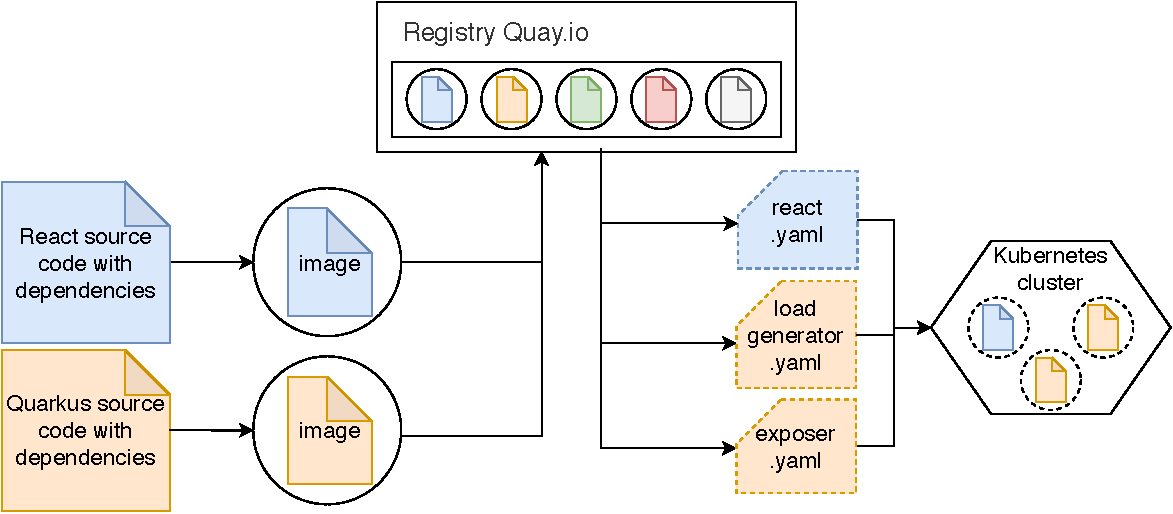
\includegraphics[width=1\linewidth]{images/03-externalSystem/deploymentOfApp.pdf}
	\caption{Process of deployment application without Strimzi using external registries}
	\label{fig:externalSystem:applicationProcess}
\end{figure}

%--------------------------------------------------------
\section{Verification phase}

The verification phase of this system is a little bit complicated. We need to think about how can we guarantee that Strizmi's behavior is working as excepted? The first idea can be checking each message that is sent to the Strimzi and every single message that is retrieved. If we imagine now that we will simulate load equality to generate one hundred thousand messages per second, that would be hard to achieve it. The different idea could be that we will be checking logs and the status of the whole application. In the Kubernetes world, we will just check pod, custom resource statuses and some metrics which can be exported by Kafka. This approach can be effortlessly delivered compared to the first scenario.

Moreover, we need to take into consideration the following steps to create a pipeline with the following stages:
\begin{itemize}
	\item \textbf{automation} \---\ point can be covered by \href{https://junit.org/junit5/}{Junit5 framework}
	\item \textbf{kubernetes client} \---\ creating abstract Kubernetes client, which will encapsulate CLI client commands to use it in java code
	\item \textbf{reporting} \---\ to be able to access this logs via top-level with the help of Jenkins \footnote{CI/CD tool https://jenkins.io/}  tool
\end{itemize}

\begin{figure*}[h!t]
	\centering
	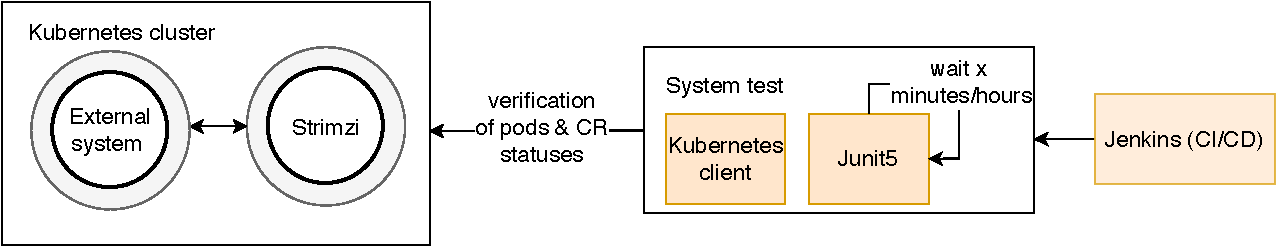
\includegraphics[width=0.9\linewidth]{images/04-verifcationPhase/VerificationBigBig.pdf}
	\caption{Process of the designed system test}
	\label{fig:verification:test}
\end{figure*}

Furthermore, designed system tests also from my perspective marathon tests. The goal of these types of tests is found bugs in the product that can only be found in long term testing.  One of the test cases is that we deploy a whole application with the Strimzi and periodically every 30 minutes checking the status of pods with also additional detailed information about Kafka resources.  A load of generating messages can be parametrized and set by environment variables inside the load generator container.  In general, these tests should run around one week to have some impact and informal value. Following figure \ref{fig:verification:test} shows these steps.

%--------------------------------------------------------
%--------------------------------------------------------
%--------------------------------------------------------
%--------------------------------------------------------
\section{Conclusions}
\label{sec:Conclusions}

In this paper, we have formulated an argument about why it is the most suitable alternative to creating your system to demonstrate user conditions instead of picking some existing ones. 

We have explained the most competent technologies used for real-time processing data inside the container environment.  Besides that, we have described core notions of Apache Kafka, such as producer, consumer, Kafka broker. Also, for the Kubernetes, we explained concepts like kube-apiserver, pod, deployment, and ultimately services.  

Moreover, we have told the whole design of the external system, which will demonstrate user conditions with different workloads. 

Lastly, we discuss the verification phase, where specifically application was tested by marathon tests. In other words, Strimzi was under some load for an extended period of time to be concrete for one week.

In the future, I have plans to extend this system to make it more parametrized. Use external storage, for instance \href{https://debezium.io/}{Debezium} \cite{Debezium}. 


\section*{Acknowledgements}
I would like to thank my supervisors, Ing. Jakub Stejskal and Mgr. Adam Rogalewicz, Ph.D. for their time. This work is realized in cooperation with Red Hat Czech, s.r.o.

%--------------------------------------------------------
%--------------------------------------------------------
%--------------------------------------------------------
%	REFERENCE LIST
%--------------------------------------------------------
%--------------------------------------------------------
\phantomsection
\bibliographystyle{unsrt}
\bibliography{2020-DataProcessingWithStrimzi-bib}

%--------------------------------------------------------
%--------------------------------------------------------
%--------------------------------------------------------
\end{document}